%% -*- coding: utf-8 -*-
\documentclass[12pt,pagesize,paper=landscape,paper=192mm:108mm]{scrbook} 
%1920x1080 1280x720
\areaset[current]{192mm}{108mm}
\usepackage{calc}
\usepackage[T2A]{fontenc}
\usepackage[utf8]{inputenc}
\usepackage[english,russian]{babel}
\usepackage{microtype}
\usepackage{misccorr}
\usepackage{cmap}
%\usepackage[unicode=true]{hyperref}
\usepackage{graphicx}
\usepackage{amssymb}
\usepackage{amsmath}
%\usepackage{srcltx}
\usepackage{textcomp}
\usepackage{xspace}
%научные символы и смайлики \smiley \frownie
\usepackage{wasysym}
\usepackage{ccicons}
\begin{document}
\begin{titlepage}
  \vspace*{-2em}
  \begin{center}    
    \hspace*{3em}
    \begin{minipage}[t]{3em}
      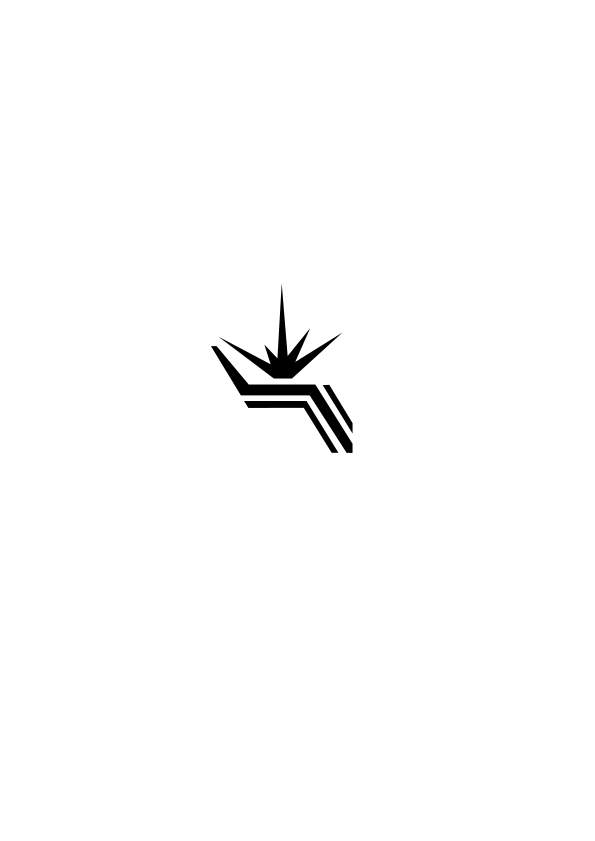
\includegraphics[width=\textwidth]{../BINP-logo}
    \end{minipage}\hfill
    \begin{minipage}{0.23\linewidth}
    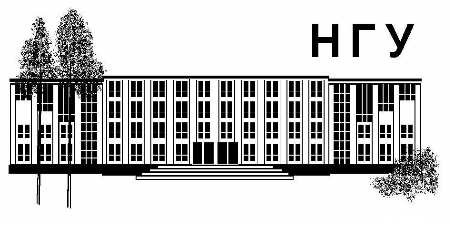
\includegraphics[width=\textwidth]{../NSU-logo}
    \end{minipage}
    \hfill
    \hspace*{6em}


    Кафедра теоретической физики физического факультета НГУ
    \medskip

    \Large
    Профессор Фадин В.\,С.

    \huge
    \textbf{Теория сильных взаимодействий}
    \smallskip
    
    \Large
    Лекция № 14
    \vfill
    
    \normalsize
    \begin{minipage}{0.9\linewidth}
      Соотношение между формфакторами $g_a$ и $h_a$. Бета"=распад
      нейтрона и экспериментальные значения $g_a$. $\pi$"=мезонный
      полюс матричного элемента аксиального тока, $f_{\pi}$, константа
      $g_{\pi NN}$. Вывод соотношения Голдбергера-Треймана (СГТ). Гипотеза
      частичного сохранения аксиального тока (ЧСАТ). Вывод СГТ из
      ЧСАТ. Кварковый конденсат. Редукционные формулы (связь матричных
      элементов с функциями Грина). Связь между массой $\pi$-мезонов,
      вакуумными конденсатами и массами $u$- и $d$"=кварков. Формула
      Гелл"=Манна"--~Окубо (массовая формула). Несколько слов о Великом
      Объединении, группа $SU(5)$.
    \end{minipage}
    \vfill
    
    \normalsize \ccbysa\hspace{0.5em}  Новосибирск 2014   
  \end{center}
\end{titlepage}
\end{document}
